\documentclass[
a4paper,
fleqn,
DIV=15,
pagesize
]{scrartcl}
\usepackage{color}
\usepackage{scrpage2}
\usepackage{subfigure}
\usepackage{booktabs}
\usepackage{enumitem}
\usepackage{graphicx}
\usepackage[utf8]{inputenc}
\usepackage{hyperref}

\graphicspath{{eps/},{../plot/}}

%\setlength{\parindent}{0pt} 

\begin{document}
\subject{MBSim -- Environment}
\title{MBSimGUI}
\subtitle{First Steps}
\author{Martin Förg}
\date{29.11.2017}

\maketitle

\begin{abstract}
This document shows first steps using the multibody simulation software
\textsc{MBSimGUI}. After installation and start a
simple model of a free falling body will be set up and simulated.
\end{abstract}

%\cleardoublepage

\tableofcontents

%\cleardoublepage

\section{Installation}
For official test releases go to \url{https://www.mbsim-env.de/mbsim/releases}
and download the newest release.
\begin{itemize}
\item On \textsc{Linux} 
download the newest *.tar.bz2 file.
Then change to the installation folder of your choice, e.\,g. your home directory
\emph{/home/dir}, and extract the archive:
\begin{verbatim}
cd /home/dir
tar xfj mbsim-env-release-x.y-linux64.tar.bz2
\end{verbatim}

\item On \textsc{Windows} 
download the newest *.zip file
and extract it to a folder of your choice, e.\,g. your home directory.
\end{itemize}

\section{Starting the GUI}

\begin{itemize}
\item On \textsc{Linux} change to the \emph{bin} folder of the new directory and start
\emph{mbsimgui}
\begin{verbatim}
cd mbsim-env/bin
mbsimgui
\end{verbatim}

\item On \textsc{Windows} 
descend to the \emph{bin} folder of the new directory and double-click on
\emph{mbsimgui.exe}.
\end{itemize}

Starting \textsc{MBSimGUI} opens a new window, the main window, as shown in figure \ref{GUI}.
\begin{figure}
\centering
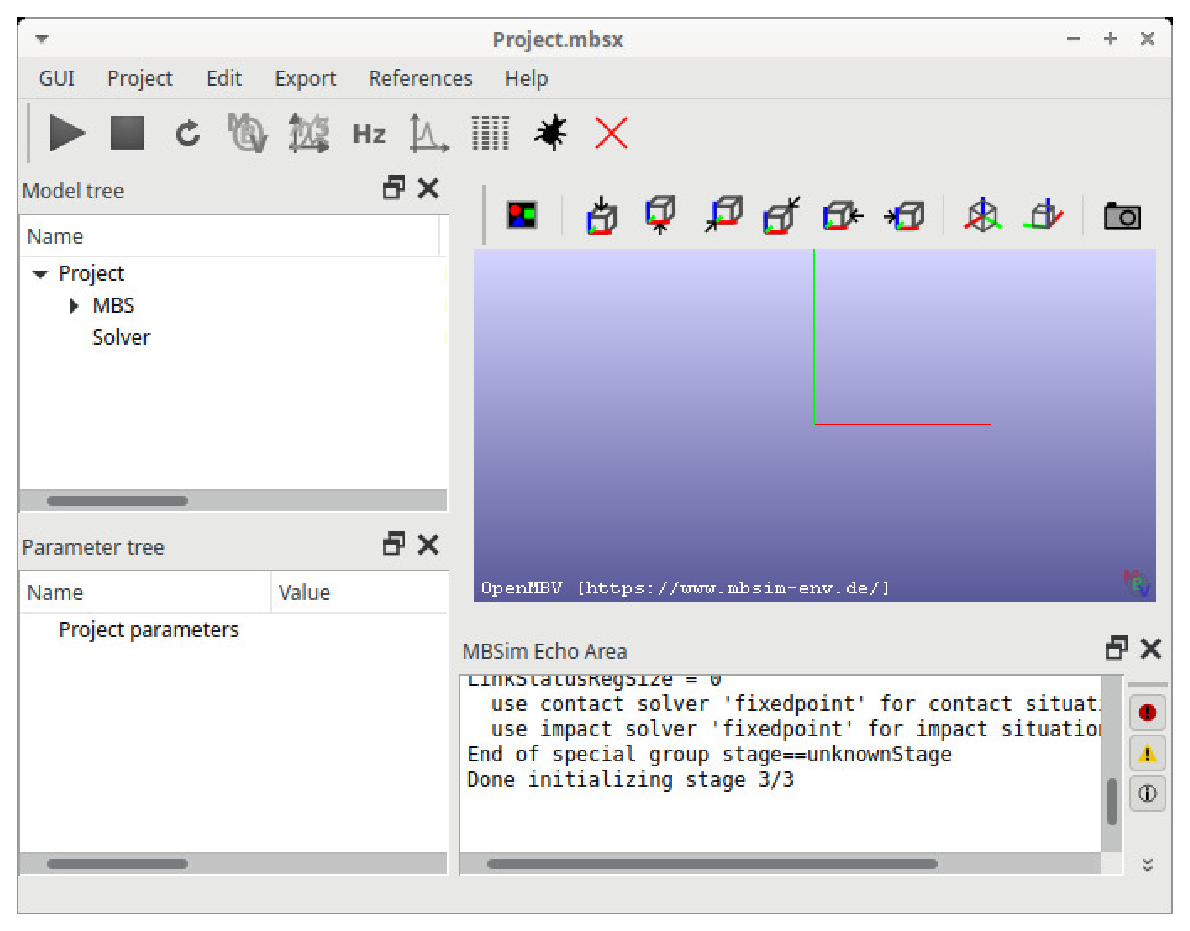
\includegraphics[scale=0.4]{GUI}
\caption{The GUI.} \label{GUI}
\end{figure}
The main window provides the following widgets:
\begin{itemize}
  \item the menu bar on top of the window allows for setting GUI options, managing
  projects and exporting project data.
  \item the buttons bar provides buttons to start and stop the simulation, to open
  the animation or the plotting tool and to debug the model.
  \item the project panel allows for setting project options.
  \item the MBS tree contains all elements of the MBS.
  It allows for adding and removing elements as well as setting their properties.
  \item the embeddings tree contains all parameters associated with an element of
  the MBS. It allows for adding and removing parameters as well as setting their
  properties.
  \item the solver panel offers different numerical solvers like integrators or
  linear system analysers.
  \item the 3D view shows the model in terms of the design of its elements. The
  view on the MBS can be translated, rotated and zoomed.
  \item the echo area gives some informations to the simulation process and shows
  possible model errors.
\end{itemize}

Currently only one element exists within the MBS. It is the inertial frame named
"I" which is always the starting point of your modeling. All absolute values to
be defined or calculated are related to this frame. The different colors refer
to the axes {\color{red} x}, {\color{green} y} and {\color{blue} z} of the
coordinate system.

To change the view on the MBS you can use one of the standard view buttons or
just press one of the three mouse buttons while moving the mouse within the 3D
view. For rotation use the left, for translation the right and for zoom the
middle mouse button.

\section{A simple example}
Now we are going to simulate a free fall. By default gravitation is enabled
acting along the negative {\color{green}y-axis}. 

First, we will add a body with a DOF along the {\color{green}y-axis}.  For this,
left-click on the arrow next to the element "MBS" to open the MBS tree.
Right-click on the container named "objects" shows a context menu. From there
choose "Add body" and then "Add rigid body".

A properties dialog opens for setting the body's data. Go to the tab named
"Kinematics", activate "Translation" and choose "Translation along y axis" from
the drop down list (figure \ref{rigidbody:prop}). Press the "OK" button to
apply the change and to close the dialog. In the 3D view a blue body should
appear (figure \ref{rigidbody:view}).
\begin{figure}
\centering
\subfigure[Property dialog of the rigid body.]{
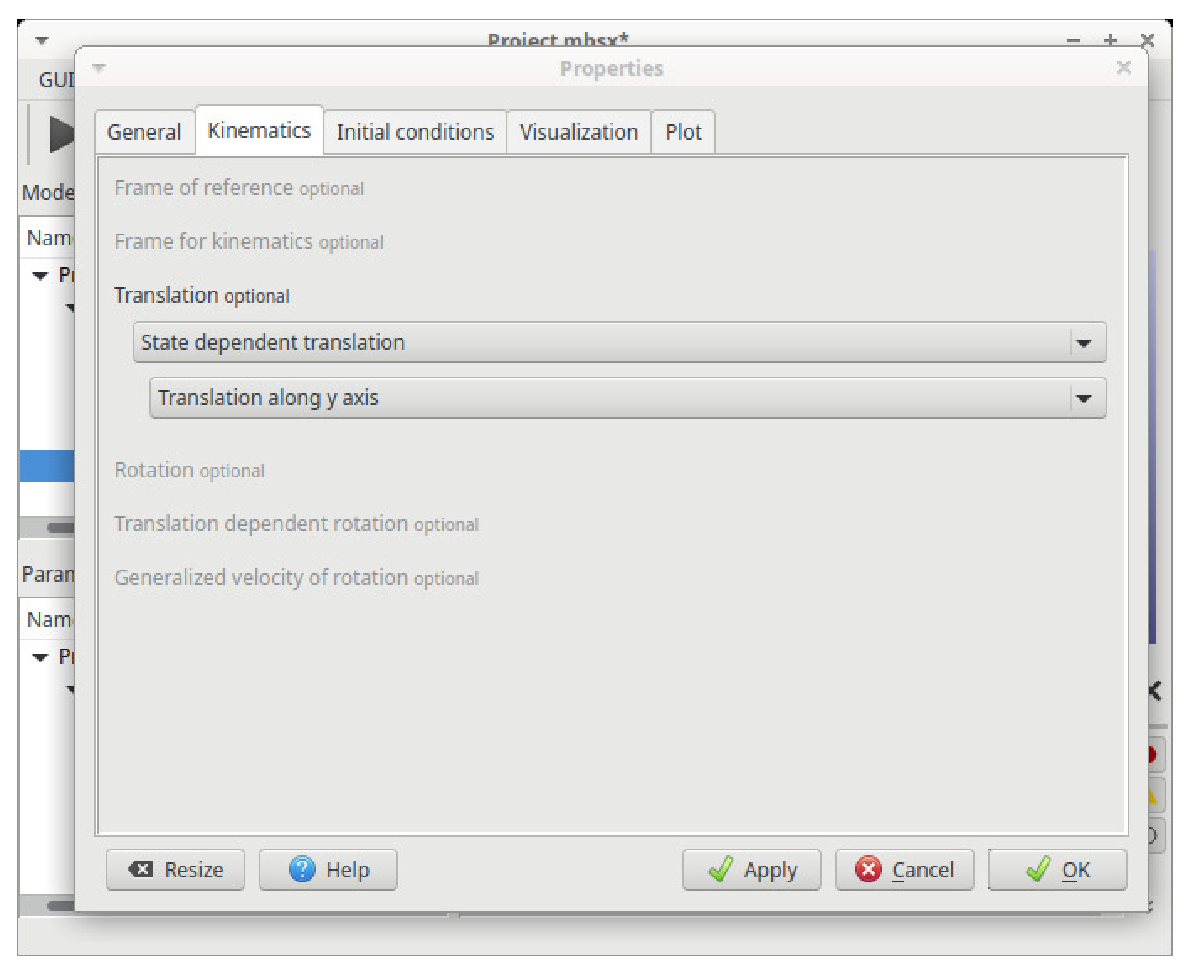
\includegraphics[scale=0.4]{kinematics} \label{rigidbody:prop}
}
\subfigure[3D view of the rigid body.]{
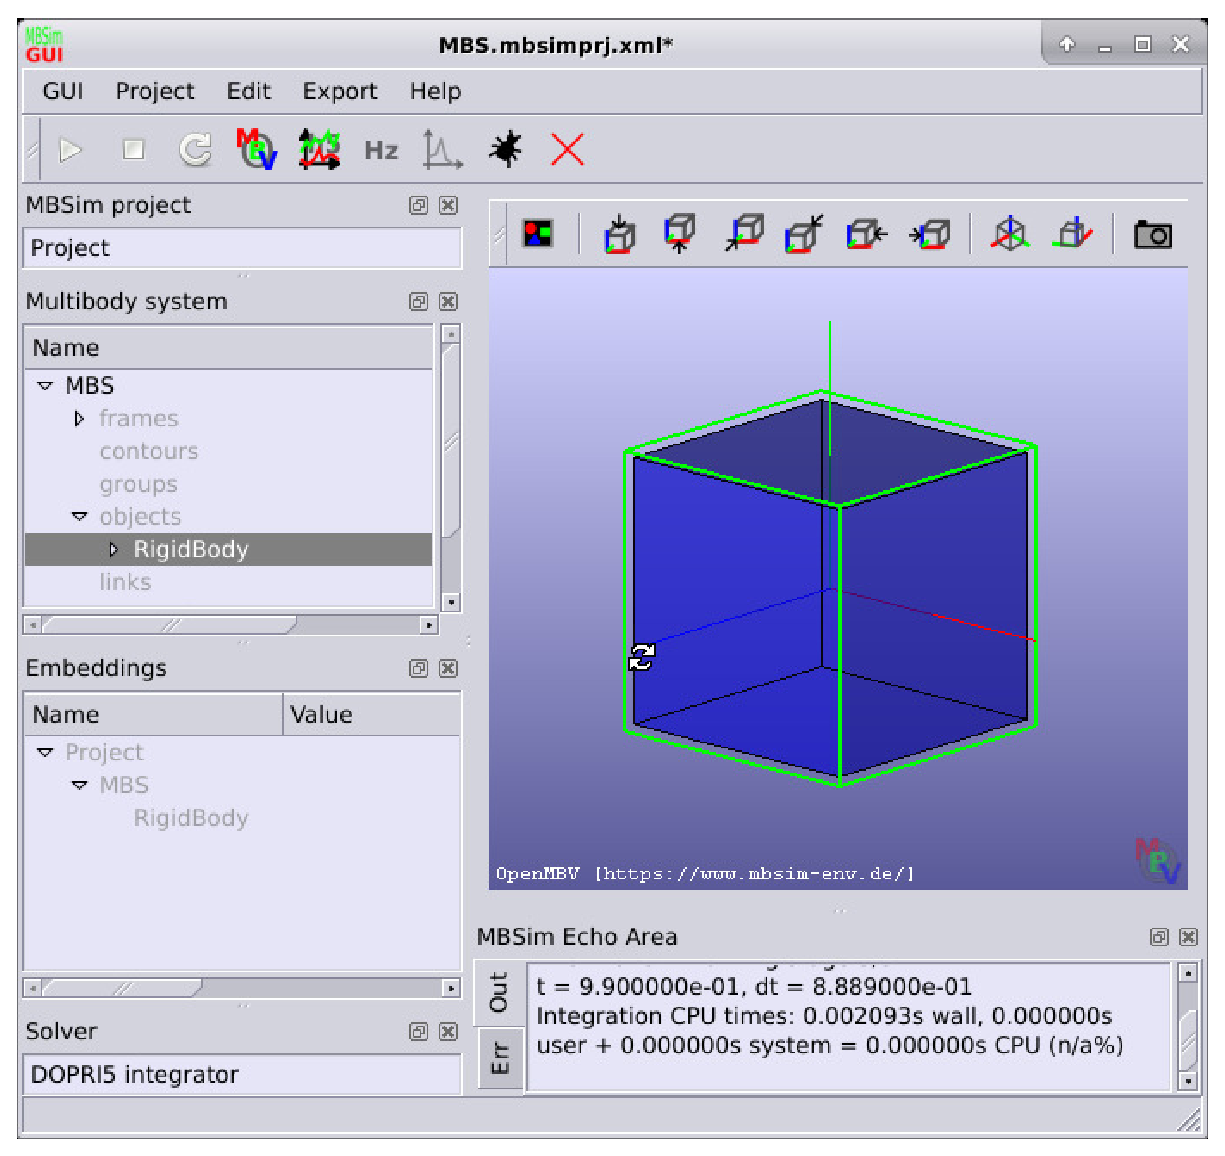
\includegraphics[scale=0.4]{body} \label{rigidbody:view}
}
\caption{Adding a rigid body to the MBS.} \label{rigidbody}
\end{figure}

Now, push the "Start simulation" button, which is the most left button in the
buttons bar. After the simulation is finished we can animate the body's
motion using \textsc{OpenMBV}.

Push the "OpenMBV" button in the middle of the buttons bar to start
\textsc{OpenMBV}.
\begin{figure}
\centering
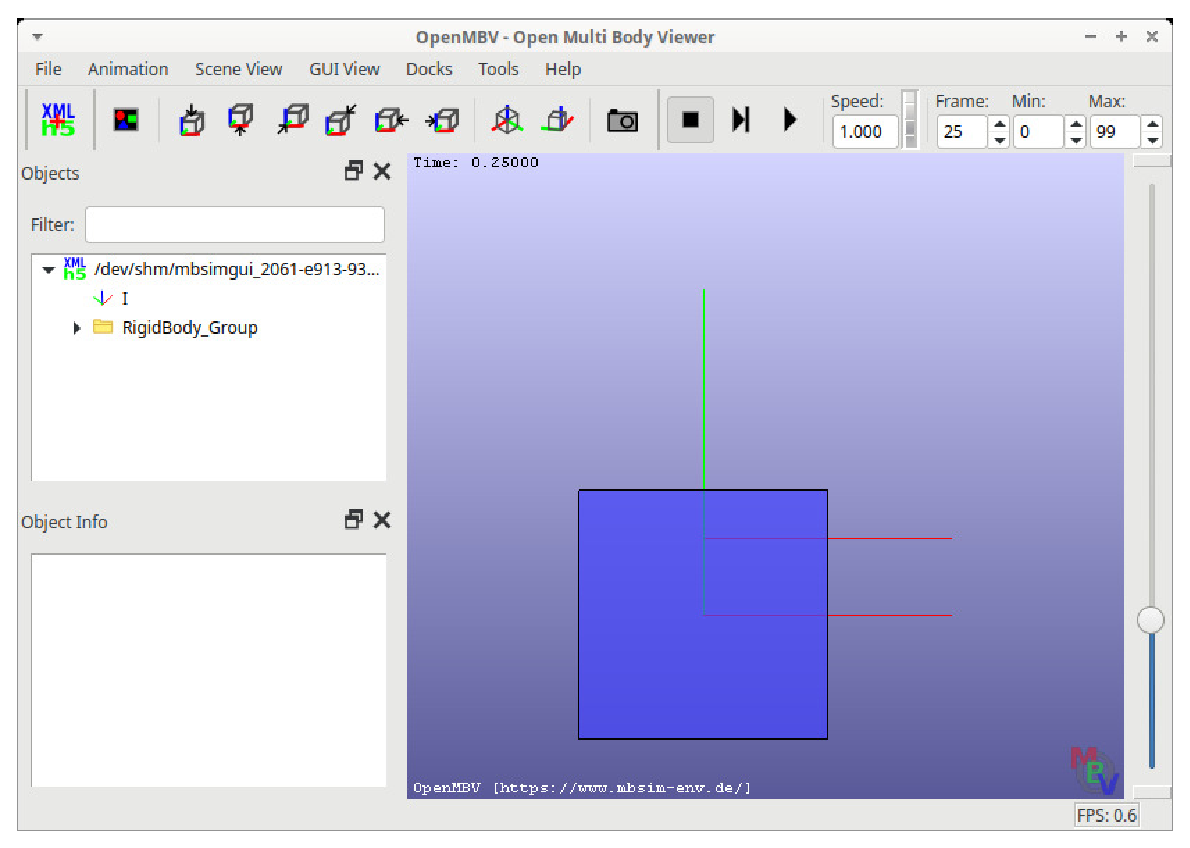
\includegraphics[scale=0.4]{openmbv}
\caption{The animation tool \textsc{OpenMBV}.} \label{openmbv}
\end{figure}
For animation click
the most right button in the buttons bar named "Run". We see the body falling
along the {\color{green}y-axis} of the inertial coordinate system (figure
\ref{openmbv}).
  
\end{document}
